\documentclass[../main.tex]{subfiles}
\graphicspath{{\subfix{../img/}}}

\begin{document}

\section{Materials and Methods} \label{sec:materials_and_methods}

\noindent\textbf{Neuronal Models}

Single-compartment conductance-based models were used to describe neuronal activity. These models explicitly describe
interactions between the membrane potential and ionic currents. The temporal dynamics of the membrane potential (i.e. potential difference between extracellular and intracellular space) is governed by the following differential equation:
\begin{equation}\label{eq:sum_currents_and_membrane_potential}
    c_m\frac{dV}{dt} = -\sum_{C} I_{C}(\vec{x}_C, V, [\text{ion}]_i; [\text{ion}]_o, g) + I_{\text{ext}}(t)
\end{equation}
where $V$ denotes the membrane potential, $c_m$ is the membrane capatience, $I_c$ is the ionic current through the ion channel $C$, and $I_{\text{ext}}$ is the external current to the neuron.

The biological background and the modelling of ion channels are described in more detail in Sections \ref{subsec:ion_channels} and \ref{subsec:modeling_ion_channels}, respectively. In short,
the ionic current depends on membrane potential $V$, extra- and intracellular concentrations of the ion to which the channel is permeable ($[\text{ion}]_i$ and $[\text{ion}]_o$, respectively), the maximal conductance $g$, and the gating variables $\vec{x}_C(V,[Ca]_i)=(m^p(V,[Ca]_i),h^q(V,[Ca]_i))$. Here, $m$ and $h$ represent activation and inactivation gate variables, and $p$ and $q$ are the respective numbers of gates. Each gating variable may depend on membrane potential $V$ and/or intracellular calcium concentration $[Ca]_i$. 

Generally, extracellular ion concentration is considered to be constant, while across different models, the intracellular ion concentration may be treated as a variable or as a constant. The maximal conductance $g$ reflects the concentration of ion channels across the membrane. 

Note that ionic currents in Equation \ref{eq:sum_currents_and_membrane_potential} are not explicitly expressed in terms of the reversal potential $V_{rev}$ (membrane potential where the current reverses direction). As discussed in Section \ref{sec:sleep_and_r5_network}, $V_{rev}$ can be estimated from the intra- and extracellular ion concentrations.

The calcium dynamics is generally modelled by a first-order differential equation of the form:
\begin{equation}
    \frac{d[Ca]_i}{dt}=f(\sum I_{Ca})
\end{equation}
where $\sum I_{Ca}$ denotes the sum over all calcium currents incorporated in the model and $f$ is a function that converts the calcium current to the calcium concentration. Examples of calcium dynamics implemented in the models are provided in Appendix \ref{appendix:functions_and_parameters}.

In this thesis, four different parameter sets were investigated across three different single-compartment conductance-based models. 
In the context of the thesis, the difference of primary interest between these models and parameter sets lies in the maximal conductances of the calcium and calcium-activated potassium channels, and their influence on membrane potential dynamics.
Figure \ref{fig:model_conductances} summarises the maximal conductances and their relative values for each of the four parameter sets. The motivation for selecting each model is discussed in Section \ref{subsec:results_preface}, and the parameter values are provided in Appendix \ref{appendix:functions_and_parameters}.


\begin{figure}[!t]
    \centering
    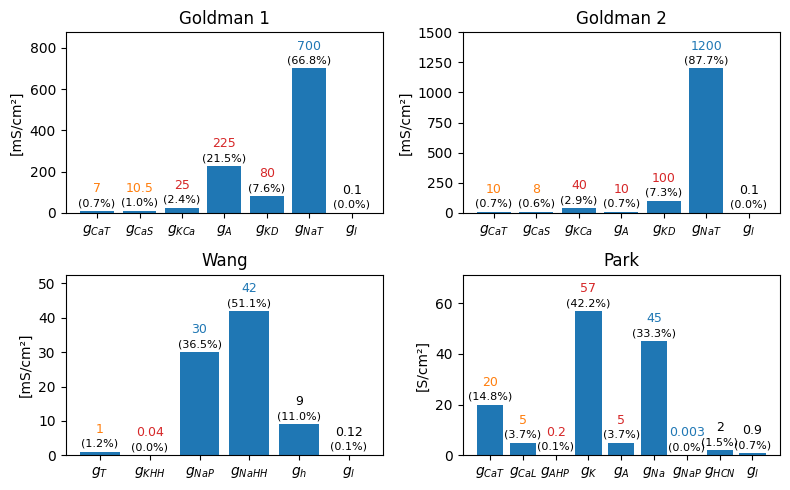
\includegraphics[width=\linewidth]{../img/materials_and_methods/model_conductances.png}
    \caption[Default maximal conductances of the models described]{
        \textbf{Default maximal conductances of the models described.} Labels on the $x$ axis correspond to ion channel names as described in the respective models (see Appendix \ref{appendix:functions_and_parameters} for a detailed description of the models).
        The numbers above each bar indicate the corresponding maximal conductance values, while the percentages below represent their relative value compared to all other channels in the same model.
        Colours indicate the ion permeability of each channel: orange for calcium, red for potassium, blue for sodium, and black for other currents (h-current and leak).
        Among all channels, the \textbf{T-type calcium channels} (labelled as \textbf{CaT} in Goldman and Park models, and \textbf{T} in the Wang model), and \textbf{calcium-activated potassium channel} (labelled as \textbf{KCa} in the Goldman models and \textbf{AHP} in the Park model) are of particular interest in the context of this work. Note that the original Wang model does not include a calcium-activated potassium channel.
    }
    \label{fig:model_conductances}
\end{figure}


%%%%%%%%%%%%%%%%%%%%%%%%%%%%%%%%%%%%%%%%%%%%%%%
\vspace*{0.3cm}
\noindent\textbf{Simulations.}

Numerical integration was performed using the Python 3.10 package '\textit{scipy.integrate.solve\_ivp}' with integration method set to LSODA. LSODA adaptively switches between stiff and nonstiff integration methods, depending on the stiffness of the system at a given time point \parencite{petzoldAutomaticSelectionMethods1983}. Initial simulations showed that the method is relatively fast in comparison to the forward Euler or RK45 method, and it was used throughout the work.

The initial condition for the membrane potential was set to $-65$mV. All other variables, including gating variables and intracellular ion concentrations, were initialised at their steady-state values.
Each simulation covered $40$ seconds of simulation time. The step size was adaptively chosen by the LSODA algorithm described above. The first 20 seconds were excluded from the analysis to allow the system to reach a stable dynamical regime. Further analysis was done on a 20-40s range of simulations.

\vspace*{0.3cm}
\noindent\textbf{Measures.}

To extract spikes from simulated membrane potential, the local maximums of the voltage trace were extracted from the simulation results using the Python package '\textit{scipy.signal.find\_peaks}'. As subthreshold oscillations are not the focus of the current thesis, the system was considered to be at rest if the range of the membrane potential ($V_{\text{max}}-V_{\text{min}}$) remained below $10$mV. This resulted in identifying time points at which spikes occurred, referred to as spiketrains.

Distribution of \gls{isi} (distance between two consecutive spikes measured in ms) was obtained from the spiketrain. The neuron was considered to be bursting if
\begin{equation*}
    min (ISI) * 3 < max(ISI)
\end{equation*}
The measure is similar to the one used in \parencite{franciRobustTunableBursting2018} and assumes that during bursting, the intraburst interval (distance between two consecutive spikes within one burst) is much larger than the interburst interval (distance between two bursts).

Burst width was defined as the average temporal distance between the first and the last spike within one burst.


\vspace*{0.3cm}
\noindent\textbf{Bifurcation Analysis.}

Bifurcation analysis was done using \textsc{AUTO-07p} \parencite{article} - a Python interface to AUTO. AAUTO is a semi-analytical tool that can be used to compute the fixed points and limit cycles, assess their stability, or track bifurcations in a dynamical system with respect to the bifurcation parameter.

In the fast–slow decomposition approach, the slow variable was treated as a bifurcation parameter.
Using the \textsc{AUTO-07p} for each value of the slow variable, the fixed points and bifurcations of the fast subsystem (system after removing the slow variable) were computed, and their stability was determined. In particular, Hopf and saddle-node bifurcations, as well as stable and unstable periodic orbits, were identified.

\end{document}